

\begin{figure}[t]
  \centerline{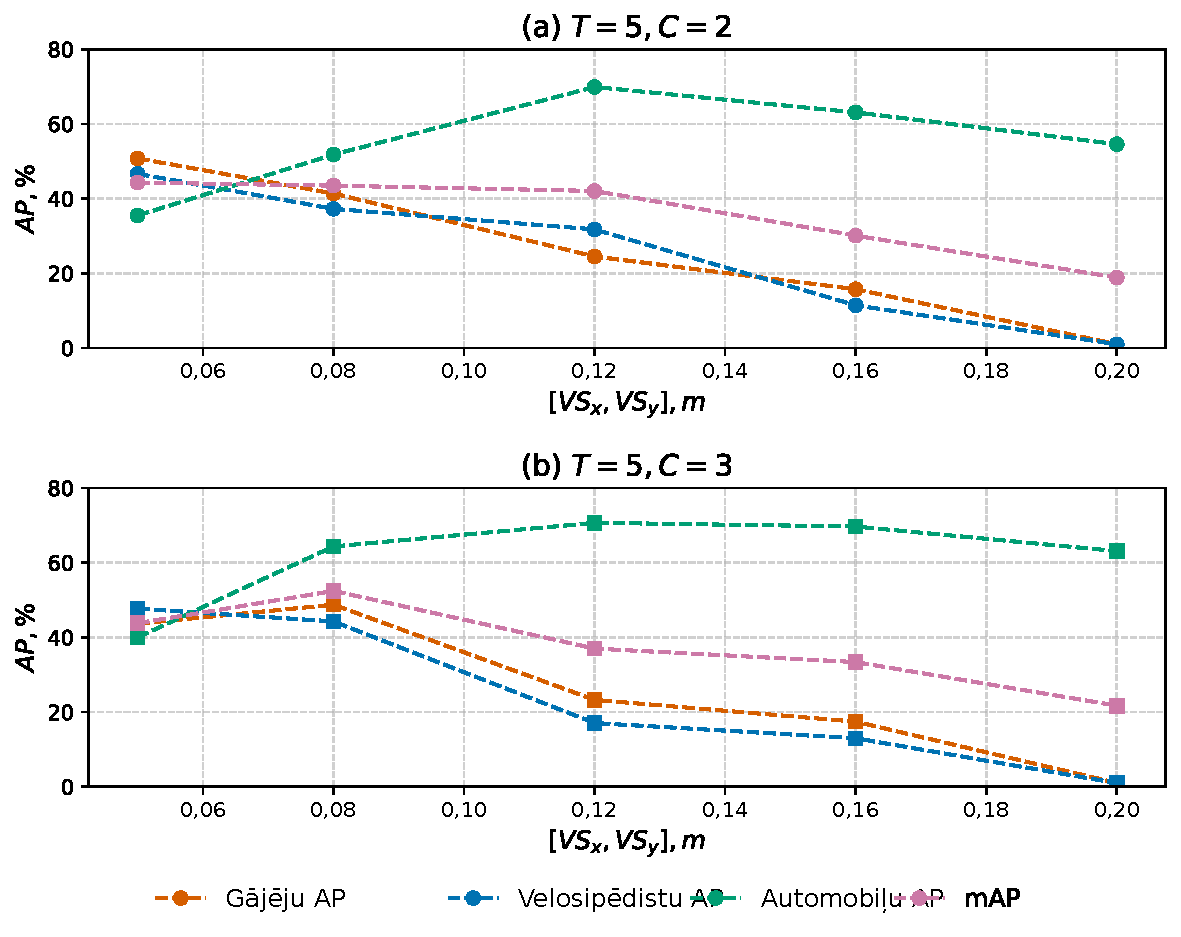
\includegraphics[width=0.75\textwidth]{fig/lv/voxel_size_chart_pretty.pdf}}
  \caption{Vokseļa izmēra ietekme uz vidējo precizitāti (AP), izmantojot impulsu VGG-11 pamattīklu ar (a) \(T=5\) laika soļiem un \(C=2\) kanāliem katrā laika solī; (b) \(T=5\) laika soļiem un \(C=3\) kanāliem katrā laika solī.}
  \label{fig:vox_size}
\end{figure}

\begin{table}[b]
\centering
\caption{Parametru skaita, retinājuma un vidējās precizitātes (\%) salīdzinājums dažādiem modeļiem}
\label{tab:detection_sparsity}
\footnotesize
\begin{adjustbox}{max width=\textwidth}\begin{tabular}{@{}lccccc@{}}
\toprule
Metode         & Param. sk. & Retinājums & Automobilis   & Gājējs & Velosipēdists \\ \midrule
Zhou u.\,c. \cite{Zhou2020} & -       & 56{,}24~\%    & 66{,}99 & 33{,}03      & 51{,}59  \\
Zhou u.\,c. \cite{Zhou2020} ar SC & -       & 56{,}24~\%    & 68{,}27 & 42{,}99      & \textbf{61{,}22}  \\ \midrule
VGG-11 (C=2)    & 12{,}8M & \textbf{55{,}73~\%}    & 63{,}09 & \textbf{50{,}77}      & 46{,}65  \\
VGG-11 (C=3)    & 12{,}8M & 59{,}56~\%    & 69{,}68 & 48{,}76      & 47{,}70  \\
VGG-13 (C=2)    & 13{,}1M & 65{,}62~\%    & 70{,}63 & 49{,}48      & 54{,}38  \\
VGG-13 (C=3)    & 13{,}1M & 63{,}67~\%    & \textbf{72{,}31} & 48{,}82      & 60{,}82  \\
\bottomrule
\end{tabular}\end{adjustbox}
\end{table}

\begin{table}[t]
\centering
\caption{Vidējās precizitātes AP salīdzinājums skatā no augšas BEV (\%) KITTI validācijas datu kopā}
\label{tab:avg-precision}
\tiny
\begin{adjustbox}{max width=\textwidth}\begin{tabular}{@{}llccccccccc@{}}
\toprule
\multirow{2}{*}{Metode} & \multirow{2}{*}{Reprezentācija} & \multicolumn{3}{c}{Automobilis} & \multicolumn{3}{c}{Gājējs} & \multicolumn{3}{c}{Velosipēdists} \\ \cmidrule(l){3-11} 
                & & Viegls      & Vidējs  & Sarežģīts & Viegls      & Vidējs  & Sarežģīts & Viegls      & Vidējs  & Sarežģīts     \\ \midrule
\textbf{Tradicionālie} &  &  &  &  &  &  &  &  &  &  \\
VoxelNet \cite{zhou2018} & Vokseļi & 89{,}35 & 79{,}26 & 77{,}39 & 46{,}13 & 40{,}74 & 38{,}11 & 66{,}7 & 54{,}76 & 50{,}55 \\
PointStabi \cite{lang2019} & Stabi & 90{,}07 & 86{,}56 & 82{,}81 & 57{,}60 & 48{,}64 & 45{,}78 & 79{,}90 & 62{,}73 & 55{,}58 \\
TANet \cite{liu2020} & Stabi & 91{,}58 & 86{,}54 & 81{,}19 & \textbf{60{,}85} & \textbf{51{,}38} & \textbf{47{,}54} & 79{,}16 & 63{,}77 & 56{,}21 \\
PointRCNN \cite{shi2019} & Punkti & 86{,}96 & 75{,}64 & 70{,}70 & 47{,}98 & 39{,}37 & 36{,}01 & 74{,}96 & 58{,}82 & 52{,}53 \\
STD \cite{yang2019} & Punkti & 94{,}74 & 89{,}19 & \textbf{86{,}42} & 60{,}02 & 48{,}72 & 44{,}55 & 81{,}36 & 67{,}23 & 59{,}35 \\
3DSSD \cite{yang2020} & Punkti & 92{,}66 & 89{,}02 & 85{,}86 & 60{,}54 & 49{,}94 & 45{,}73 & \textbf{85{,}04} & 67{,}62 & 61{,}14 \\
PV-RCNN \cite{shi2020} & Punkti+vokseļi & \textbf{94{,}98} & \textbf{90{,}65} & 86{,}14 & 59{,}86 & 50{,}57 & 46{,}74 & 82{,}49 & \textbf{68{,}89} & \textbf{62{,}41}  \\
\midrule \midrule
\textbf{Uz SNN balstītie} &  &  &  &  &  &  &  &  &  &  \\
\cite{Zhou2020} bez SC & Vokseļi & 68{,}94 & 66{,}65 & 65{,}39 & 38{,}03 & 32{,}43 & 28{,}64 & 58{,}40 & 50{,}61 & 45{,}75 \\
\cite{Zhou2020} ar SC & Vokseļi & 71{,}76 & 67{,}43 & 65{,}63 & 47{,}07 & 42{,}53 & 39{,}36 & 69{,}16 & 59{,}24 & 55{,}25 \\
Šis darbs VGG-11(C=3) & Vokseļi & 73{,}52 & 68{,}64 & 66{,}88 & 50{,}42 & 49{,}75 & 46{,}10 & 44{,}05	& 45{,}35 & 43{,}37\\
Šis darbs VGG-13(C=3) & Vokseļi & 76{,}11 & 72{,}03 & 68{,}80 & 51{,}43 & 49{,}23 & 45{,}79 & 62{,}75 & 61{,}11 & 58{,}61\\
\bottomrule
\end{tabular}\end{adjustbox}
\end{table}

Kā ilustrēts \ref{fig:vox_size}. attēlā (a) ar \(C=2\), vokseļa izmēra izvēle būtiski ietekmē impulsu \textit{VGG-11} modeļa
vidējo precizitāti. Tas norāda, cik svarīgi ir saglabāt mazu šūnas izmēru, lai mazākos mērogos atšķirtu gājēju un
velosipēdistu klases. Savukārt lielākiem automobiļu objektiem vokseļa izmēra samazināšana ne vienmēr uzlabo precizitāti.
\ref{fig:vox_size}. attēlā (b) vertikālā izšķirtspēja efektīvi palielināta, palielinot kanālu skaitu līdz 3 un nemainot laika
soļu skaitu, tādējādi panākot ievērojamu automobiļu detektēšanas vidējās precizitātes uzlabojumu par 6,59~\%. Process
atkārtots impulsu \textit{VGG-13} detektēšanas pamattīklam, un abu modeļu rezultāti sniegti \ref{tab:detection_sparsity}.
tabulā. Palielinot tīkla dziļumu, novērojama līdzīga atkarība no vokseļa izmēra, vienlaikus sasniedzot augstāku vidējo
precizitāti uz lielāku realizācijas izmaksu rēķina. Piemēram, izmantojot 2 kanālus katrā laika solī un saglabājot tādu pašu
šūnas izmēru, velosipēdistu klasei uzlabojums ir 7,73~\% un automobiļu klasei 7,54~\%. Salīdzinājumā ar cieši saistītu
\Gls{snn}
risinājumu darbā \cite{Zhou2020} šī pieeja vairumā gadījumu sasniedz labāku veiktspēju pat bez šī darbā realizētiem
izlaides savienojumiem, tikai nedaudz atpaliekot velosipēdistu kategorijā.

Jāatzīmē arī, ka specializētās aparatūras sistēmās impulsi tiek izstaroti un pārraidīti uz nākamajiem slāņiem tikai tad, kad
neirona membrāna sasniedz noteiktu slieksni. Neironu impulsu ģenerēšanas dinamikas izpratne ir būtiska maksimālas aprēķinu
efektivitātes sasniegšanai. Retinājumu izmanto kā slāņa aktīvo neironu īpatsvara mēru, kas atspoguļo tīkla aktivitātes
sadalījumu. \ref{tab:detection_sparsity}. tabulā sniegti visā datu kopā vidējoti retinājuma mērījumi kopā ar modeļa parametru
skaitu un vidējo precizitāti. Starp tiem \textit{VGG-11} realizācijai ir zemāks retinājuma rādītājs 55,73~\%, kas ir
līdzīgā līmenī ar salīdzināto risinājumu.

Rezultāti, kas iegūti ar \(C=3\) kanāliem katrā laika solī, salīdzinājumā ar izvēlētām tradicionālām \Gls{ann} arhitektūrām sniegti
\ref{tab:avg-precision}. tabulā. Lai gan šī risinājums ir mazāk precīzs nekā sarežģītāki \Gls{ann} modeļi, tā veiktspēja ir
konkurētspējīga ar dažām vienkāršākām tradicionālajām pieejām, īpaši gājēju detektēšanā. Ar \textit{VGG-13} sasniegtā klašu
vidējā precizitāte attiecīgi 63,43~\%, 60,79~\% un 57,73~\% vieglajā, vidējā un sarežģītajā kategorijā pārspēj tikai
\textit{VoxelNet}, \textit{PointRCNN} un līdzvērtīgus modeļus, galvenokārt zemākas automobiļu klases detektēšanas
precizitātes dēļ. Tomēr galvenais arguments \Gls{snn} izmantošanai ir reta apstrāde, kas balstās tikai uz \Gls{acc}
operācijām tradicionālas blīvas apstrādes ar \Gls{mac} operācijām vietā.

Lai gan būtu jāveic plaši papildu eksperimenti ar
neiromorfo aparatūru, lai kritiski izvērtētu apgalvojumus par mazu jaudas patēriņu, jaunākajos pētījumos impulsu \textit{VGG}
energoefektivitāte novērtēta analītiski \cite{dampfhoffer2022}. Izmantojot darba \cite{dampfhoffer2022} metodoloģiju,
tradicionālo \Gls{cnn} un \Gls{snn} patērēto enerģiju var novērtēt attiecīgi ar (\ref{eq:eann}) un (\ref{eq:esnn}). Relatīvās
enerģijas izmaksas pieņemtas atbilstoši darbam \cite{dampfhoffer2022} \qty{45}{\nano\metre} \Gls{cmos} tehnoloģijai.
% \textit{VGG-11} un \textit{VGG-13} topoloģiju attiecības ir attiecīgi \(N_{syn/neur}=\) \num{9.0e2} un \num{9.9e2}. Ar
% \(T=5\) laika soļiem un \(N_{spikes/syn}=1\) iegūst \(E_{ANN}/E_{SNN}=\)1,378 un 1,379 reizes lielāku energoefektivitāti
% attiecīgi \textit{VGG-11} un \textit{VGG-13} salīdzinājumā ar ekvivalentu \Gls{ann} modeli.
% Kā secināts darbā \cite{dampfhoffer2022}, energoefektivitātei ir būtiski saglabāt mazu laika soļu skaitu. Tomēr ar mazāku
% laika soļu skaitu enerģijas patēriņā dominē atmiņas lasīšanas un rakstīšanas operācijas sinapsēs, jo \(N_{syn} \times
% N_{spikes/syn} >> N_{neur} \times T\). Pat ar \(T=10\) laika soļiem energoefektivitāte samazinās nenozīmīgi 1,004 reizes.
% Šajā darbā izmantotajai modeļa topoloģijai tikai turpmāka \(N_{spikes/syn}\) samazināšana varētu būtiski uzlabot
% energoefektivitāti salīdzinājumā ar \Gls{ann}.
Novērtējuma rezultāti apkopoti \ref{tab:snn_energy_comparison}. tabulā. VGG-11 un VGG-13 arhitektūru vidējās sinapšu un neironu
skaita attiecības \(N_{\mathrm{syn}}/N_{\mathrm{neur}}\) ir attiecīgi \num{9.0e2} un \num{9.9e2}. Pieņemot \(T=5\)
simulācijas laika soļus un vidēji \(N_{\mathrm{spikes/syn}}=1\) impulsu uz vienu sinapsi visā inferenču laika intervālā,
saskaņā ar (\ref{eq:delta_e}) aprēķinātais \Gls{snn} arhitektūru enerģijas patēriņš ir attiecīgi par 27,43\% un 27,48\%
mazāks nekā ekvivalentajiem \Gls{ann} modeļiem.
Kā secināts pētījumā \cite{dampfhoffer2022}, neliels simulācijas laika soļu skaits ir būtisks energoefektivitātes
nodrošināšanai. Tomēr pie neliela laika soļu skaita enerģijas patēriņā dominē ar sinaptiskajām operācijām saistītās atmiņas
lasīšanas un rakstīšanas operācijas, jo \(N_{\mathrm{syn}} \times N_{\mathrm{spikes/syn}} \gg N_{\mathrm{neur}} \times T\).
Tādējādi simulācijas laika soļu skaita palielināšana var samazināt energoefektivitātes priekšrocību.
Palielinot simulācijas laika soļu skaitu no \(T=5\) līdz \(T=10\) un saglabājot \(N_{\mathrm{spikes/syn}}=1\), aprēķinātais
enerģijas patēriņš palielinājās tikai par 0,4\%. Šāds salīdzinoši neliels pieaugums ir skaidrojams ar novērtēto arhitektūru
lielo sinapšu un neironu skaita attiecību, kuras dēļ enerģijas modelī dominē sinaptiskās operācijas un ar tām saistītās
atmiņas piekļuves. Tādēļ aplūkotajās arhitektūrās būtiskāku enerģijas patēriņa samazinājumu attiecībā pret \Gls{ann} modeļiem
varētu panākt, samazinot vidējo impulsu skaitu uz vienu sinapsi \(N_{\mathrm{spikes/syn}}\).

\begin{table}[t]
\centering
\caption{Pulsējošu VGG arhitektūru analītiski novērtētais enerģijas patēriņa samazinājums salīdzinājumā ar ekvivalentajiem ANN
  modeļiem pie \(T=5\).}
\label{tab:snn_energy_comparison}
\begin{tabular}{lcc}
\toprule
\textbf{Arhitektūra} &
\(\boldsymbol{N_{\mathrm{syn}}/N_{\mathrm{neur}}}\) &
\textbf{Enerģijas patēriņa} \\
& & \textbf{samazinājums (\%)} \\
\midrule
VGG-11 & \num{9.0e2} & 27,43 \\
VGG-13 & \num{9.9e2} & 27,48 \\
\bottomrule
\end{tabular}
\end{table}
